% Copyright (c) 2022 by Lars Spreng
% This work is licensed under the Creative Commons Attribution 4.0 International License. 
% To view a copy of this license, visit http://creativecommons.org/licenses/by/4.0/ or send a letter to Creative Commons, PO Box 1866, Mountain View, CA 94042, USA.

%~~~~~~~~~~~~~~~~~~~~~~~~~~~~~~~~~~~~~~~~~~~~~~~~~~~~~~~~~~~~~~~~~~~~~~~~~~~~~~
% You can add your packages and commands to the loadslides.tex file. 
% The files in the folder "styles" can be modified to change the layout and design of your slides.
% I have included examples on how to use the template below. 
% Some of these examples are taken from the Metropolis template.
%~~~~~~~~~~~~~~~~~~~~~~~~~~~~~~~~~~~~~~~~~~~~~~~~~~~~~~~~~~~~~~~~~~~~~~~~~~~~~~


\documentclass[
11pt,notheorems,hyperref={pdfauthor=Hyunseong Kim}
]{beamer}

\usepackage{graphicx}       % graphics
\graphicspath{{media/}}     % organize your images and other figures under media/ folder
\newcommand{\braket}[2]{\left \langle #1 \middle| #2 \right \rangle}
\newcommand{\braketmatrix}[3]{\left \langle #1 \middle| #2 \middle| #3 \right \rangle}
\usepackage{braket}
\usepackage{tikz}
\usetikzlibrary{quantikz2}
\usepackage{pgf}
\usepackage{pgfmath}
\usetikzlibrary{shapes.geometric, math}

% Copyright (c) 2022 by Lars Spreng
% This work is licensed under the Creative Commons Attribution 4.0 International License. 
% To view a copy of this license, visit http://creativecommons.org/licenses/by/4.0/ or send a letter to Creative Commons, PO Box 1866, Mountain View, CA 94042, USA.

%~~~~~~~~~~~~~~~~~~~~~~~~~~~~~~~~~~~~~~~~~~~~~~~~~~~~~~~~~~~~~~~~~~~~~~~~~~~~~~
% Add your packages and commands to this file
%~~~~~~~~~~~~~~~~~~~~~~~~~~~~~~~~~~~~~~~~~~~~~~~~~~~~~~~~~~~~~~~~~~~~~~~~~~~~~~

%~~~~~~~~~~~~~~~~~~~~~~~~~~~~~~~~~~~~~~~~~~~~~~~~~~~~~~~~~~~~~~~~~~~~~~~~~~~~~~
% Fonts
% \RequirePackage{palatino} % for serif slides
% \usefonttheme{serif}
\RequirePackage[scaled]{helvet} % for sans-serif slides

\RequirePackage[utf8]{inputenc}
\RequirePackage[T1]{fontenc}


\usepackage{styles/elegantmacros}
\usefolder{styles}
\usetheme[style=lecture]{elegant}

\newcommand{\makepart}[1]{ % For convenience
\part{#1} \frame{\partpage}
}

%~~~~~~~~~~~~~~~~~~~~~~~~~~~~~~~~~~~~~~~~~~~~~~~~~~~~~~~~~~~~~~~~~~~~~~~~~~~~~~

%~~~~~~~~~~~~~~~~~~~~~~~~~~~~~~~~~~~~~~~~~~~~~~~~~~~~~~~~~~~~~~~~~~~~~~~~~~~~~~
% Figures
\RequirePackage{booktabs}
\RequirePackage{colortbl}
\RequirePackage{ragged2e}
\RequirePackage{schemabloc}
%\RequirePackage{natbib}
\RequirePackage{caption}
\RequirePackage{subcaption}
\RequirePackage{tabularx}
\RequirePackage{array}
\RequirePackage{multirow}
\RequirePackage[%
  natbib=true, backend=biber,%
  style=apa, isbn=false,url=false,uniquename=false%, useprefix=true%
  ]{biblatex}
\addbibresource{references.bib}
\newcolumntype{Y}{>{\centering\arraybackslash}X}

%~~~~~~~~~~~~~~~~~~~~~~~~~~~~~~~~~~~~~~~~~~~~~~~~~~~~~~~~~~~~~~~~~~~~~~~~~~~~~~

%~~~~~~~~~~~~~~~~~~~~~~~~~~~~~~~~~~~~~~~~~~~~~~~~~~~~~~~~~~~~~~~~~~~~~~~~~~~~~~
% Figures
\RequirePackage{wrapfig}
\RequirePackage{pgfplots}
\RequirePackage{graphicx}
\RequirePackage{adjustbox}
\RequirePackage{environ}
\pgfplotsset{compat=1.18}

\makeatletter
\newsavebox{\measure@tikzpicture}
\NewEnviron{scaletikzpicturetowidth}[1]{%
  \def\tikz@width{#1}%
  \def\tikzscale{1}\begin{lrbox}{\measure@tikzpicture}%
  \BODY
  \end{lrbox}%
  \pgfmathparse{#1/\wd\measure@tikzpicture}%
  \edef\tikzscale{\pgfmathresult}%
  \BODY
}
\makeatother
%~~~~~~~~~~~~~~~~~~~~~~~~~~~~~~~~~~~~~~~~~~~~~~~~~~~~~~~~~~~~~~~~~~~~~~~~~~~~~~

%~~~~~~~~~~~~~~~~~~~~~~~~~~~~~~~~~~~~~~~~~~~~~~~~~~~~~~~~~~~~~~~~~~~~~~~~~~~~~~
% Maths 
\RequirePackage{textcomp}
\RequirePackage{amsmath} 
\RequirePackage{amsthm}
\RequirePackage{mathtools}
%\RequirePackage{bbm}
%\RequirePackage{algorithm}
%\RequirePackage[osf,sc]{mathpazo}
%\RequirePackage{pifont}
%\newcommand{\xmark}{\ding{55}}%
%\numberwithin{equation}{section}
\DeclareMathOperator*{\argmax}{arg\,max}
\DeclareMathOperator*{\argmin}{arg\,min}

\setbeamertemplate{theorems}[numbered] % to number

\theoremstyle{definition}
\newtheorem{fact}{Fact}[section]
\newtheorem{examp}{Example}[section]

\theoremstyle{plain}
\newtheorem{definition}{Definition}[section]
\newtheorem{proposition}{Proposition}
\newtheorem{theorem}{Theorem}
\newtheorem{assumption}{Assumption}

\providecommand{\H}{\mathscr{H}}      
\providecommand{\E}{\mathbb{E}}
\makeatletter
\def\munderbar#1{\underline{\sbox\tw@{$#1$}\dp\tw@\z@\box\tw@}}
\makeatother

%~~~~~~~~~~~~~~~~~~~~~~~~~~~~~~~~~~~~~~~~~~~~~~~~~~~~~~~~~~~~~~~~~~~~~~~~~~~~~~
 % Loads packages and some defined commands

\title[
    
% Text entered here will appear in the bottom middle
]{Trotter Circuit Optimization}

\subtitle{through Adiabatic computation}

\author[
% Text entered here will appear in the bottom left corner
]{
    Kim, Hyunseong
}

\institute{
    Quantum Field and Gravity Theory Group, \\
    GIST, Department of Physics and Photonics}
\date{August 31, 2023}

\begin{document}

% Generate title page
{
\setbeamertemplate{footline}{} 
\begin{frame}
  \titlepage
\end{frame}
}
\addtocounter{framenumber}{-1}

% You can declare different parts as a parentof sections
\begin{frame}
    \tableofcontents[part=1]
\end{frame}

\makepart{QUBO problems in circuit optimization}
\section{Lie-Trotter Formula and Circuit}

\subsection{Trotterization}
\begin{frame}
    To simulate time-evolving process such as adiabatic quantum process,
    we approximate continuous process with discrete steps. 
    
    We call the discretized approximation as \textbf{Trotter} formula.
    
    \begin{equation}
        \label{eq:trotter}
        \exp(- i \mathcal{H} t) \approx \Pi_i^n \exp\left(- i \mathcal{H}_i \frac{t}{n}\right)
    \end{equation}

    where, $n$ is a trotter steps. 
    
    As we increase the step number $n$, we get more precise unitary trnasformation.
\end{frame}

\begin{frame}
    Practically, each terms of Hamiltonian are described with \textbf{Pauli string}.
    A single Pauli string, for example $XZIY$, Hamiltonian has a well known corresponding circuit.
    
    \begin{equation}
        \exp(- i \Delta t  (X \otimes Z \otimes I \otimes Y))
    \end{equation}

    \begin{figure}
        \begin{quantikz}
            \gate{H}  &         & \ctrl{3} &         &                       &          & \ctrl{3}& \gate{H}&\\
                      &         &          &\ctrl{2} &                       & \ctrl{2} &         &         &\\
                      &         &          &         &                       &          &         &         &\\
            \gate{H} &\gate{S}  & \targ{}  & \targ{} & \gate{R_Z(2 \Delta t)}& \targ{}  & \targ{} & \gate{S^\dagger} & \gate{H}
        \end{quantikz}
    \end{figure}
\end{frame}

\section{Optimization of Hamiltonian}
\begin{frame}
    Optimization of evolution circuit is a combination of two parts.

    \begin{itemize}
        \item Mutually Commuting Partition 
        \item Pauli-Frame
    \end{itemize}
\end{frame}
\subsection{Mutually Commuting Partition}
\begin{frame}
    Pauli strings are always anti-commute or commute each other.

    For given two Pauli strings, $P_i, P_j$,
    \begin{equation}
        \text{either }\, [P_i, P_j] =0 \, \text{or} \, \{P_i, P_j\} =0
    \end{equation}

    where, $[\,]$ is a commutator, and $\{\,\}$ is an anti-commutator.

    If all Pauli-terms of Hamiltonain are mutually commute each other, 
        Eq(\ref{eq:trotter}) becomes an unitary operator of total Hamiltonain evolution of time $t$.

        \begin{equation}
            \exp(- i \mathcal{H} t) = \Pi_i^n \exp\left(-i \mathcal{H}_i t \right)
        \end{equation}
\end{frame}

\begin{frame}

    \begin{enumerate}
        \item We must know all commuting relation of the given Pauli-stirng set.
        \item How to make a mutually partitions of the given set?
    \end{enumerate}

\end{frame}

\begin{frame}
    To make a mutually commuting partition, we have to know all commuting relationships of the given Pauli-terms of Hamiltonian.
    We can check the commutation with General commutativity(GC), see \cite{9248636}.
    
    If a system is $n$ qubits system and there are $m$ number of Pauli-terms, total operation would be, roughly,

    \begin{equation}
        {m \choose 2} * n = O(m^2 n)
    \end{equation}

    Unfortunately, $\max(m) = 2^n$ for $n$-qubit system Hamiltonian, it could be expoentially growth.
\end{frame}

\begin{frame}
    \cite{chapuis_finding_2018} suggested acceleration of commuting term determination. 

    They decompose single Pauli-string into $X$ and $Z$ families. 

    \begin{itemize}
        \item $X$-family: $IIIX, XIXI, IIXI, XXII, IXXX, \dots$
        \item $Z$-family: $IIIZ, ZIZI, IIZI, ZZII, IZZZ, \dots$
    \end{itemize}

    \begin{equation}
        YZIX = XIIX \cdot ZZII = x_i \cdot z_j
    \end{equation}

    \begin{equation}
        [P_i, P_j] = [x_k z_l, x_m, z_n] = 
        \begin{cases} 
            0 & if [z_l, x_m] = [x_k, z_n]\\
            -2P_i P_j & otherwise 
         \end{cases}
    \end{equation}
\end{frame}

\begin{frame}
    Now, if we have compatible grpah of Pauli-set,
    we can extract mutually commuting partition by solving a sequential Max-Clique problem of the commute graph.

    It is well known NP-complete problem, from 21-complete problems. See \cite{Karp1972}. %https://link.springer.com/chapter/10.1007/978-1-4684-2001-2_9
    


    \cite{doi:10.1021/acs.jpca.2c06453} suggested Ising formulation for finding Max-clique finding problem of compatible graph.

    \begin{equation}
        \mathcal{H} = - \mu_0 \sum Z_i + \mu_1 \sum h_{ij} Z_i Z_j
    \end{equation}

    where, $h_{ij} = 0$ if $Z_i -Z_j$ edge weight is $0$ otherwise 1, $\mu_0 = 1, \mu_1 =2$ in Kurita et al.. 
\end{frame}

\begin{frame}
    \begin{figure}[ht]
        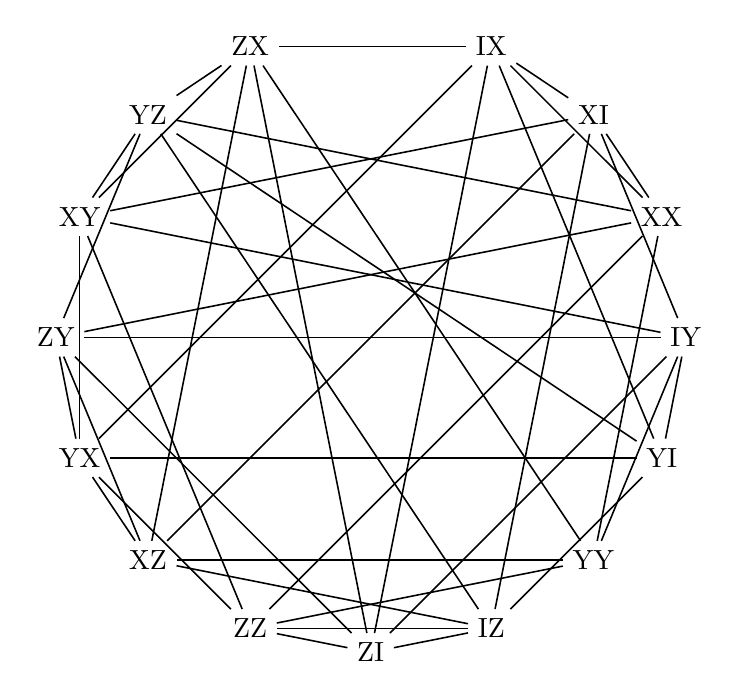
\begin{tikzpicture}
            \node[] (IX) at (2*0.7653668647301797 , 2* 1.847759065022573)    {IX};
            \node[] (XI) at (2*1.4142135623730951 , 2*1.414213562373095)    {XI};
            \node[] (XX) at (2*1.8477590650225735 , 2*0.7653668647301796)   {XX};
            \node[] (IY) at (2*2.0, 0.0)                                  {IY};
            \node[] (YI) at (2* 1.847759065022573 , 2*-0.7653668647301808)   {YI};
            \node[] (YY) at (2* 1.4142135623730947 , 2*-1.4142135623730954)  {YY};
            \node[] (IZ) at (2* 0.76536686473018 , 2*-1.8477590650225733)    {IZ};
            \node[] (ZI) at (2* 0 , 2*-2.0)                                  {ZI};
            \node[] (ZZ) at (2* -0.7653668647301807 , 2*-1.847759065022573)  {ZZ};
            \node[] (XZ) at (2* -1.4142135623730954 , 2*-1.414213562373095)  {XZ};
            \node[] (YX) at (2* -1.8477590650225737 , 2*-0.7653668647301793) {YX};
            \node[] (ZY) at (2* -2.0 , 2*0)                                  {ZY};
            \node[] (XY) at (2* -1.8477590650225735 , 2*0.7653668647301798)  {XY};
            \node[] (YZ) at (2* -1.414213562373095 , 2*1.4142135623730951)   {YZ};
            \node[] (ZX) at (2* -0.7653668647301795 , 2*1.8477590650225735)  {ZX};

            \draw[line width=0.2mm, black ,-] (IX) -- (ZX) ;
            \draw[line width=0.2mm, black ,-] (IX) -- (YX) ;
            \draw[line width=0.2mm, black ,-] (IX) -- (ZI) ;
            \draw[line width=0.2mm, black ,-] (IX) -- (YI) ;
            \draw[line width=0.2mm, black ,-] (IX) -- (XX) ;
            \draw[line width=0.2mm, black ,-] (IX) -- (XI) ;

            \draw[line width=0.2mm, black ,-] (XI) -- (XY) ;
            \draw[line width=0.2mm, black ,-] (XI) -- (XZ) ;
            \draw[line width=0.2mm, black ,-] (XI) -- (IZ) ;
            \draw[line width=0.2mm, black ,-] (XI) -- (IY) ;
            \draw[line width=0.2mm, black ,-] (XI) -- (XX) ;

            \draw[line width=0.2mm, black ,-] (XX) -- (YZ);
            \draw[line width=0.2mm, black ,-] (XX) -- (ZY);
            \draw[line width=0.2mm, black ,-] (XX) -- (ZZ);
            \draw[line width=0.2mm, black ,-] (XX) -- (YY);

            \draw[line width=0.2mm, black ,-] (IY) -- (XY);
            \draw[line width=0.2mm, black ,-] (IY) -- (ZY);
            \draw[line width=0.2mm, black ,-] (IY) -- (ZI);
            \draw[line width=0.2mm, black ,-] (IY) -- (YY);
            \draw[line width=0.2mm, black ,-] (IY) -- (YI);

            \draw[line width=0.2mm, black ,-] (YI) -- (YZ);
            \draw[line width=0.2mm, black ,-] (YI) -- (YX);
            \draw[line width=0.2mm, black ,-] (YI) -- (IZ);

            \draw[line width=0.2mm, black ,-] (YY) -- (ZX);
            \draw[line width=0.2mm, black ,-] (YY) -- (XZ);
            \draw[line width=0.2mm, black ,-] (YY) -- (ZZ);

            \draw[line width=0.2mm, black ,-] (IZ) -- (YZ);
            \draw[line width=0.2mm, black ,-] (IZ) -- (XZ);
            \draw[line width=0.2mm, black ,-] (IZ) -- (ZZ);
            \draw[line width=0.2mm, black ,-] (IZ) -- (ZI);

            \draw[line width=0.2mm, black ,-] (ZI) -- (ZX);
            \draw[line width=0.2mm, black ,-] (ZI) -- (ZY);
            \draw[line width=0.2mm, black ,-] (ZI) -- (ZZ);
            
            \draw[line width=0.2mm, black ,-] (ZZ) -- (XY);
            \draw[line width=0.2mm, black ,-] (ZZ) -- (YX);
        

            \draw[line width=0.2mm, black ,-] (XZ) -- (ZX);
            \draw[line width=0.2mm, black ,-] (XZ) -- (ZY);
            \draw[line width=0.2mm, black ,-] (XZ) -- (YX);

            \draw[line width=0.2mm, black ,-] (YX) -- (XY);
            \draw[line width=0.2mm, black ,-] (YX) -- (ZY);

            \draw[line width=0.2mm, black ,-] (ZY) -- (YZ);

            \draw[line width=0.2mm, black ,-] (XY) -- (ZX);
            \draw[line width=0.2mm, black ,-] (XY) -- (YZ);

            \draw[line width=0.2mm, black ,-] (ZX) -- (YZ);
        \end{tikzpicture}
    \end{figure}
\end{frame}

\begin{frame}
    \begin{figure}[ht]
        \begin{tikzpicture}
            \node[] (IX) at (2*0.7653668647301797 , 2* 1.847759065022573)    {IX};
            \node[] (XI) at (2*1.4142135623730951 , 2*1.414213562373095)    {XI};
            \node[] (XX) at (2*1.8477590650225735 , 2*0.7653668647301796)   {XX};
            \node[] (IY) at (2*2.0, 0.0)                                  {IY};
            \node[] (YI) at (2* 1.847759065022573 , 2*-0.7653668647301808)   {YI};
            \node[] (YY) at (2* 1.4142135623730947 , 2*-1.4142135623730954)  {YY};
            \node[] (IZ) at (2* 0.76536686473018 , 2*-1.8477590650225733)    {IZ};
            \node[] (ZI) at (2* 0 , 2*-2.0)                                  {ZI};
            \node[] (ZZ) at (2* -0.7653668647301807 , 2*-1.847759065022573)  {ZZ};
            \node[] (XZ) at (2* -1.4142135623730954 , 2*-1.414213562373095)  {XZ};
            \node[] (YX) at (2* -1.8477590650225737 , 2*-0.7653668647301793) {YX};
            \node[] (ZY) at (2* -2.0 , 2*0)                                  {ZY};
            \node[] (XY) at (2* -1.8477590650225735 , 2*0.7653668647301798)  {XY};
            \node[] (YZ) at (2* -1.414213562373095 , 2*1.4142135623730951)   {YZ};
            \node[] (ZX) at (2* -0.7653668647301795 , 2*1.8477590650225735)  {ZX};

            \draw[line width=0.2mm, green ,-] (IX) -- (XX) ;
            \draw[line width=0.2mm, green ,-] (IX) -- (XI) ;
            \draw[line width=0.2mm, green ,-] (XI) -- (XX) ;

            \draw[line width=0.2mm, green ,-] (IY) -- (YY);
            \draw[line width=0.2mm, green ,-] (IY) -- (YI);
            \draw[line width=0.2mm, green ,-] (YI) -- (YY);

            \draw[line width=0.2mm, green ,-] (IZ) -- (ZZ);
            \draw[line width=0.2mm, green ,-] (IZ) -- (ZI);
            \draw[line width=0.2mm, green ,-] (ZI) -- (ZZ);

            \draw[line width=0.2mm, green ,-] (XZ) -- (YX);
            \draw[line width=0.2mm, green ,-] (XZ) -- (ZY);
            \draw[line width=0.2mm, green ,-] (YX) -- (ZY);


            \draw[line width=0.2mm, green ,-] (XY) -- (ZX);
            \draw[line width=0.2mm, green ,-] (XY) -- (YZ);
            \draw[line width=0.2mm, green ,-] (ZX) -- (YZ);
        \end{tikzpicture}
    \end{figure}
\end{frame}

\subsection{Pauli Frame}
\begin{frame}
    \begin{figure}
        \begin{quantikz}
            \gate{H}  &         & \ctrl{3} &         &         \gate{R_Z(\theta_1)}              &          & \ctrl{3}& \gate{H}&\\
                      &         &          &\ctrl{2} &         \gate{R_Z(\theta_2)}              & \ctrl{2} &         &         &\\
                      &         &          &         &         \gate{R_Z(\theta_3)}              &          &         &         &\\
            \gate{H} &\gate{S}  & \targ{}  & \targ{} & \gate{R_Z(2 \Delta t)}& \targ{}  & \targ{} & \gate{S^\dagger} & \gate{H}
        \end{quantikz}
    \end{figure}

    \begin{equation*}
        \mathcal{H} = t XZIY + \theta_1 XIII + \theta_2 IZII + \theta_3 IIII
    \end{equation*}
\end{frame}

\begin{frame}
\begin{figure}
    \begin{quantikz}
        \gate{H}  &         & \ctrl{1} &         &         \gate{R_Z(\theta_1)}              &          & \ctrl{1}& \gate{H}&\\
                  &         & \targ{}  &\ctrl{2} &         \gate{R_Z(\theta_2)}              & \ctrl{2} &  \targ{} &         &\\
                  &         &          &         &         \gate{R_Z(\theta_3)}              &          &         &         &\\
        \gate{H} &\gate{S}  &          & \targ{} & \gate{R_Z(2 \Delta t)}& \targ{}  &  & \gate{S^\dagger} & \gate{H}
    \end{quantikz}
    \begin{equation*}
        \mathcal{H} = t XZIY + \theta_1 XIII + \theta_2 XZII + \theta_3 IIII
    \end{equation*}
\end{figure}
\end{frame}

\begin{frame}
    \cite{schmitz_graph_2023} analyzed and Pauli-Frame method and optimized circuit with minimum cost of $CNOT, H, S$ operations to 
    \begin{equation}
        \begin{array}{cc}
            Z_1 & X_1\\
            Z_2 & X_2\\
            Z_3 & X_3\\
            Z_4 & X_4\\
        \end{array} \rightarrow_{H_2, H_4-S_4}
        \begin{array}{cc}
            X_1 & Z_1\\
            Z_2 & Z_2\\
            Z_3 & X_3\\
            Y_4 & Z_4\\
        \end{array}  \rightarrow_{CNOT{1, 2}}
        \begin{array}{cc}
            X_1 & Z_1\\
            X_1Z_2 & Z_1 X_2\\
            Z_3 & X_3\\
            Y_4 & X_4\\
        \end{array} \rightarrow_{CNOT{2, 4}}
        \begin{array}{cc}
            X_1 & Z_1\\
            X_1Z_2 & Z_1X_2\\
            Z_3 & X_3\\
            X_1 Z_2 Y_4 & Z_1 X_2 Z_4\\
        \end{array}
    \end{equation}

    \begin{figure}
        \begin{quantikz}[scale=0.5]
            \gate{H}  &         & \ctrl{1} &         &         \gate{R_Z(\theta_1)}              &          & \ctrl{1}& \gate{H}&\\
                      &         & \targ{}  &\ctrl{2} &         \gate{R_Z(\theta_2)}              & \ctrl{2} &  \targ{} &         &\\
                      &         &          &         &         \gate{R_Z(\theta_3)}              &          &         &         &\\
            \gate{H} &\gate{S}  &          & \targ{} & \gate{R_Z(2 \Delta t)}& \targ{}  &  & \gate{S^\dagger} & \gate{H}
        \end{quantikz}
        \begin{equation*}
            \mathcal{H} = t XZIY + \theta_1 XIII + \theta_2 XZII + \theta_3 IIII
        \end{equation*}
    \end{figure}
\end{frame}

\section{Degenerate Reducing of Mutually Hamiltonian}

\begin{frame}
    If there are two max clique on graph, sharing same number of nodes, the next Hamiltonian pick one of them randomly.

    \begin{equation}
        \mathcal{H} = - \mu_0 \sum Z_i + \mu_1 \sum h_{ij} Z_i Z_j
    \end{equation}

    Eventhough, they are same in commutation graph, frame change cost can be different. 

    In this project, we only consider $H, S$ costs. 
    The weight of each Pauli-terms would be calculated with function $w(,)$, such that

    \begin{itemize}
        \item $w(,) = 0$: $(X,X)$, $(Y,Y)$, $(Z,Z)$, $(Z,I)$
        \item $w(,) = 1$: $(X,Z)$,$(X,Y)$,$(X,I)$
        \item $w(,) = 2$: $(Y,I)$, $(Y,Z)$
    \end{itemize}

For $N$-qubit system, extended weight function $W(,)$ is defined as,

\begin{equation}
    \label{eq:Weight}
   W(S_i, S_j) :=  \frac{1}{N} \sum_{k=1}^N w((S_{i})_k, (S_{j})_k)
\end{equation}
\end{frame}


\begin{frame}
    \begin{figure}
        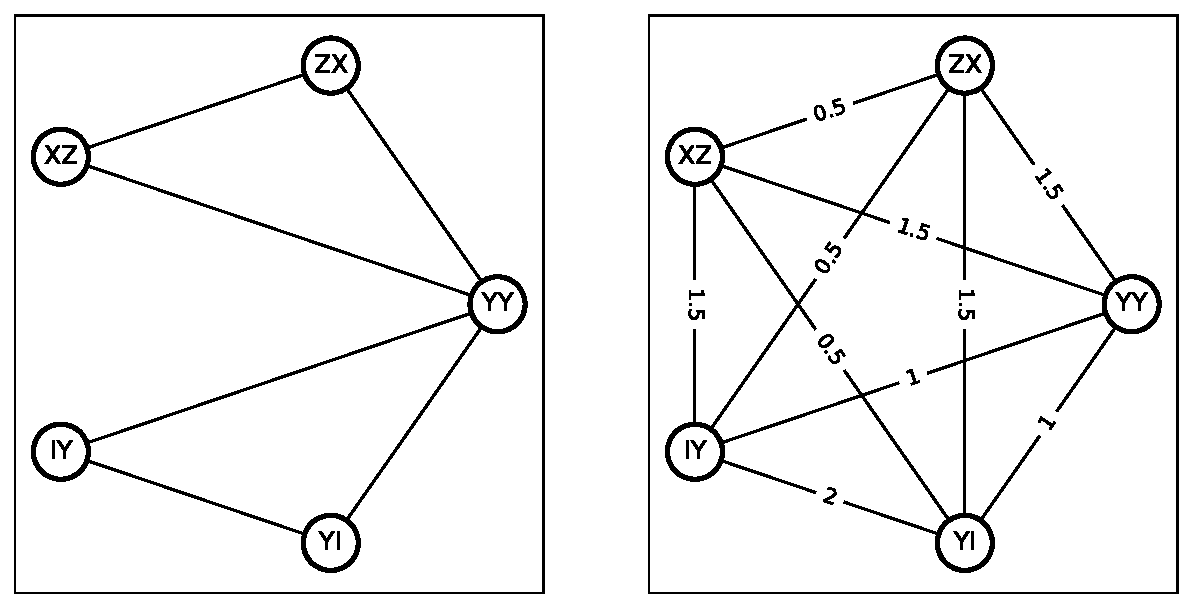
\includegraphics[scale=0.7]{degenerate.pdf}
        \caption{Compatible and basis transform weight graph example. Left graph is a compatible graph of 5 Pauli basis of 2 qubits system and edges are indicating commutation relationship. Right graph is a basis transform weight graph of the same Pauli-basis set of the left.}
    \label{fig:graph}
    \end{figure}
\end{frame}

\begin{frame}
    We can redefine a Hamiltonian for optimization,

    \begin{equation}
        \label{eq:whamiltonian}
        \mathcal{H} = - \mu_0 \sum Z_i + \mu_1 \sum_{i <j} h_{ij} Z_i Z_j + \mu_2 \sum_{i<j} w_{ij} Z_i Z_j 
    \end{equation}

    To avoid the degeneration of energy and to conserve max and commuting condition, the coefficients, $\mu_0, \mu_1, \mu_2$ have next relationship.
    
    For $N$ qubits system,

    \begin{equation}
        \|\mu_1\| > N \|\mu_0\| \,  \|\mu_0\| > \frac{1}{2} N(N-1) \|\mu_2\|
    \end{equation}

\end{frame}

\begin{frame}
    Full procedure of algorithm.

    \begin{enumerate}
        \item Find a compatible graph of the given Hamiltonian
        \item Calculate weigtht between Pauli-strings with Eq(\ref{eq:Weight})
        \item Find a min-number of mutually commuting partition, $p_1, p_2, \dots$, using \textbf{adiabatic computer}.
        \item Find a shortest hamilton path of each local partition $p_i$, <- reduced problem, you can use classic algorithm.
        \item Connecting $p_i$ in order to following 4 step result.
    \end{enumerate}
\end{frame}

\section{Optimization Example}
\subsection{HeH+ molcular hamiltonian}
\begin{frame}
    Pennylane HeH+ molcule Hamiltonian: 
    
    4 qubits are required and consist of 25 Pauli-terms.


    'ZXZX','IYIY','ZYZY','IZIZ','XZXZ','XIXI','YZYZ','YIYI','ZIZI',
 ,'IIIZ', 'ZZII', 'IZZI', 'ZIIZ', 'IZII', 'IIZI', 'ZIII', 'IIZZ',
 ,'XZXI', 'YZYI', 'XXYY', 'YXXY', 'YYXX', 'XYYX', 'IYZY', 'IXZX'


\end{frame}

\begin{frame}
    \begin{figure}
        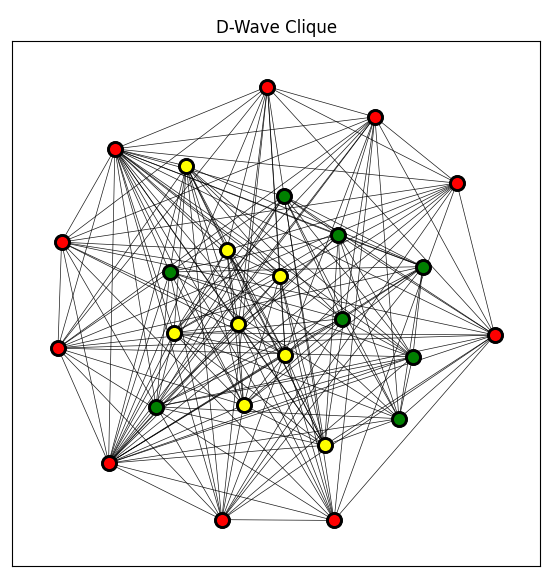
\includegraphics[scale=0.5]{clique.png}
        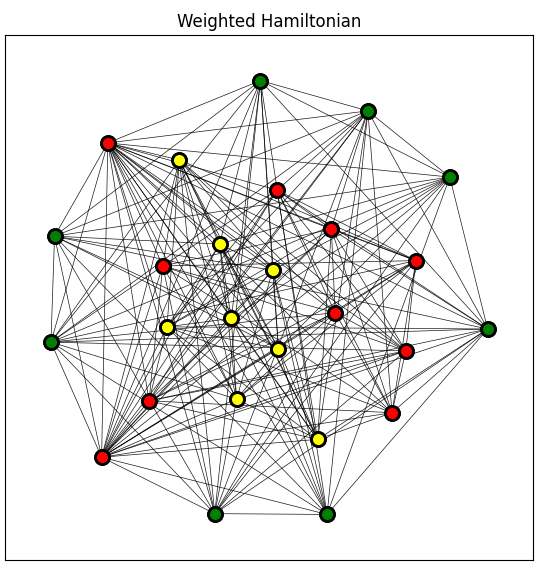
\includegraphics[scale=0.5]{clique_w.png}
        \caption{Commuting Partition HeH+ Hamiltonian Pauli-terms. Left: Ising formula solution of D-Wave. Right: Basis cost term weight added optimization.}       
    \end{figure}
\end{frame}

\begin{frame}
    The optimization result is 3 number of partition.

    $p_0$
    ['ZXZX','IYIY','ZYZY','IZIZ','XZXZ','XIXI','YZYZ','YIYI','ZIZI']
    
    $p_1$
    ['IIIZ', 'ZZII', 'IZZI', 'ZIIZ', 'IZII', 'IIZI', 'ZIII', 'IIZZ']

    $p_2$
    ['XZXI', 'YZYI', 'XXYY', 'YXXY', 'YYXX', 'XYYX', 'IYZY', 'IXZX']

\end{frame}

\begin{frame}
    \begin{figure}
        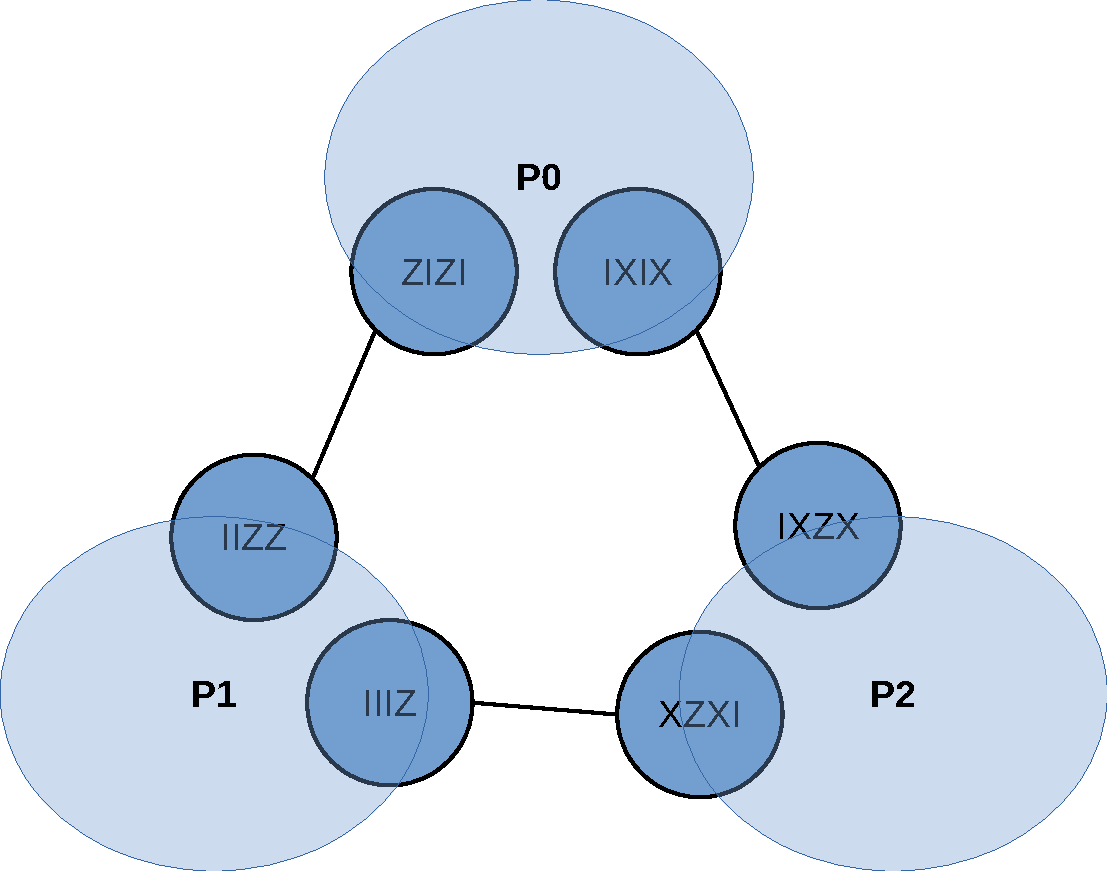
\includegraphics[scale=0.45]{ppp.pdf}
    \end{figure}
\end{frame}

\begin{frame}
    Compare to Pennylane ApproxTimeEvovle() circuit

    \begin{figure}
        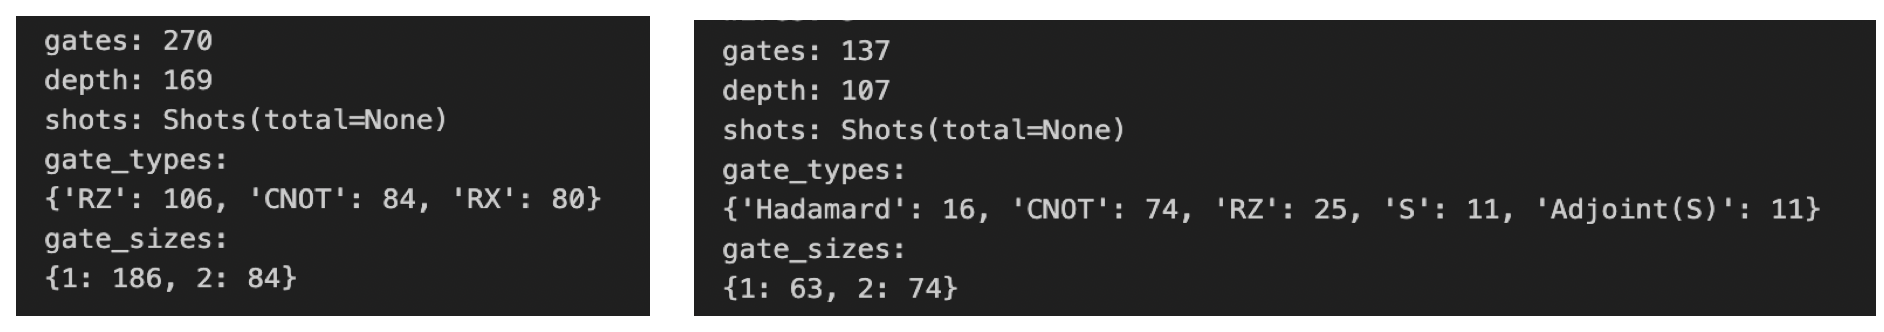
\includegraphics[scale=0.55]{compare.png}
        \caption{Left: Pennylane ApproxTimeEvolve() trotter number =1 circuit. Right: Optimized evolve circuit.}
    \end{figure}
\end{frame}


\begin{frame}[allowframebreaks]{References}
    \printbibliography
\end{frame}

\end{document}